\documentclass[../../main.tex]{subfiles}

\begin{document}

\subsection{Design}
I dette afsnit vil designprocessen for systemet blive gennemgået. Der vil i dette afsnit blive gennemgået og forklaret de processer der er benyttet, overvejelser der er blevet gjort, og de resultater der er opnået.

\subsubsection{Designmodellen}
Designmodellen i Unified Process består i, at efter dette workflow er færdigt, skal implementeringen af koden kunne udføres, da designmodellen detaljeret vil beskrive den fulde funktionalitet for Sensum Udred. Designmodel workflowet inddeles i to forskellige views. Et statisk view, som vil indeholde designklassediagrammet for Sensum Udred med implementeringsdetaljer og designrelationer. Det dynamiske view af designmodellen vil indeholde sekvensdiagrammer, såsom det arkitektoniske sekvensdiagram, og overordnede sekvensdiagram for Sensum Udred. I det statiske view vises Sensum Udreds opbygning indeholdende implementeringsdetaljer, og i det dynamiske view vises Sensum Udred i aktion med implementeringsdetaljer. Dette inkludere attributter, operationer med returtyper og parameterlister.

\paragraph{Det statiske view}\mbox{} \\
I dette afsnit beskrives det statiske view i forhold til hvilke overvejelser, beslutninger og resultater der har været. Det statiske view af designmodellen er selve designklassediagrammet, de enkelte designklasser og designrelationer i designklassediagrammet. 

\begin{figure}[H]
  \centering
  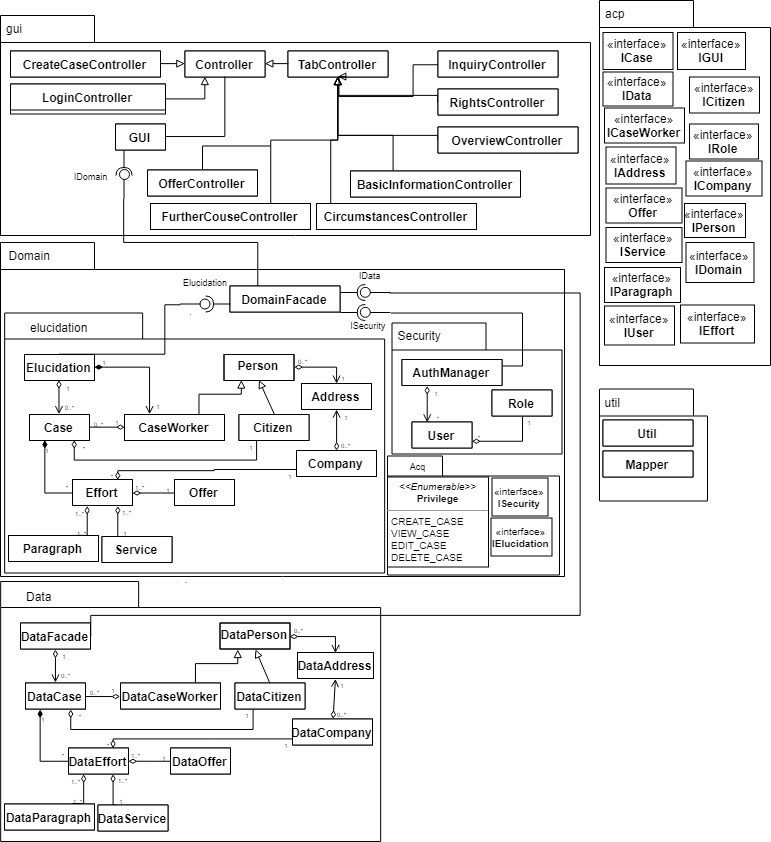
\includegraphics[scale=.45]{figurer/over-design-diagram.jpg}
  \caption{Overordnet Designklassediagram}
  \label{fig:over-designklassediagram}
\end{figure}

På figur \ref{fig:over-designklassediagram}, ses det designklassediagram der implementeres ud fra. Det fulde designklassediagram kan findes i bilag \ref{designmodel-detaljeret}. Bag dette diagram er der udført brugsmønsterrealiseringer, og iterativt blevet tilføjet implementeringsdetaljer. 

Som det kan ses ovenstående i figur \ref{fig:over-designklassediagram}, er der tilføjet \code{<<get/set>>} på private attributter. Dette er en notation, som der er valgt at bruge til at beskrive, at attributterne har public getter og setter metoder, som skal bruges for at tilgå eller sætte attributterne. I standard UML notation ville man tilføje alle getter og setter metoderne til den pågældende klasse i designmodellen, men i nogle tilfælde er der op til 20 af disse metoder. Det er derfor valgt at bruge denne notation for at holde designmodellen overskuelig. Dette er dog ikke en standard notation, som UML har implementeret. I systemets design model er det benyttet således:

\begin{itemize}
\item Privat attribut med getter og setter metode beskrives ved \code{<<get/set>>} 
\item Privat attribut med setter(mutator) metode beskrives ved \code{<<set>>}
\item Privat attribut med getter(accessor) metode beskrives ved \code{<<get>>}
\end{itemize}
\mbox{} \\
Idéen bag denne notation stammer fra et opslag på Stackoverflow.\cite{stack}

Ved overgangen fra analyseklassediagrammet til Designklassediagrammet skulle der gøres en del overvejelser for at implementeringen af koden kunne udføres på den mest optimale måde. Først og fremmest blev der overvejet hvor fyldestgørende designklassediagrammet skulle være før kodeimplementeringen kunne påbegyndes, fordi der arbejdes iterativt med designklassediagrammet igennem designmodellen. Et eksempel på tre specifikke designklasser kan ses på figur \ref{fig:komposition}. Her måtte overvejes hvorvidt at det skulle være muligt at hente attributternes værdi for en \code{Person}, men også om de senere hen skulle kunne ændres med \code{set} metoderne. Det skal være muligt at ændre personers fornavn, med mere, efter de er sat første gang, i tilfælde af ændringer i diise, og det skal også være muligt at tilgå dem. Derfor har de både fået getter og setter metoder.

Der blev først lavet et forsimplet designklassediagram, der tog udgangspunkt i brugsmønster-realiseringerne fra analysemodellen. Til at starte med blev der set bort fra interfaces, og lagt stor vægt på at lave fyldestgørende designklasser ud fra vores analyseklasser. Interfaces ville komme senere, når tre-lagsarkitekturen blev opsat. På den måde kunne der fokuseres på domæne-laget først. Udover dette blev associationer overvejet fra analyseklassemodellen. På den måde kunne de modelleres, som enten aggregeringer eller kompositioner i designklassediagrametm. Disse associationer ændrede sig dog undervejs, da ansvarsfordelingen for hvem der for eksempel oprettede Casen ændrede sig fra at være en \code{User} til at blive en \code{CaseWorker}. Dette gjorde domænelaget mere logisk og objektorienteret. En anden overvejelse var hvem der skulle oprette en instans af \code{CaseWorker}. Dette kan ses modelleret på fig \ref{fig:komposition}. Her kan det ses, at det er systemfacaden der står for at oprette en instans af \code{CaseWorker}, og den binder Caseworkeren med en \code{User}. Grunden til at relationen mellem \code{Caseworker} og \code{SystemFacade} vises med en komposition er, at det er \code{Elucidation}, der har ansvar for at oprette instansen. Så uden \code{Elucidation} ville \code{CaseWorker} ikke kunne eksistere. I forhold til GRASP, så ses \code{Elucidation}, som en creator af \code{CaseWorker}.

\begin{figure}[H]
  \centering
  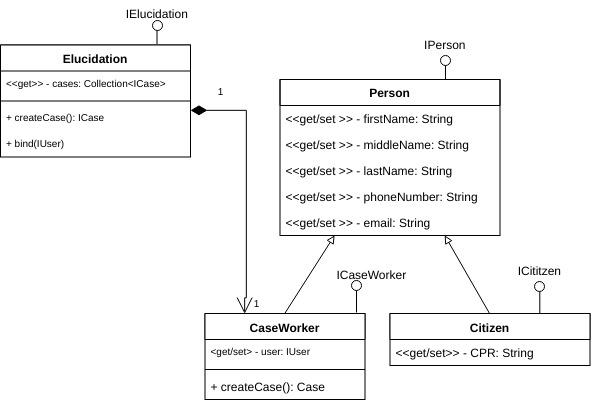
\includegraphics[scale=.4]{figurer/Komposition.jpeg}
  \caption{Modellering af komposition for Caseworker}
  \label{fig:komposition}
\end{figure}

En anden overvejelse der også blev gjort i forhold til associationer, var hvorvidt at en \code{CaseWorker} skulle kunne være tilknyttet flere sager, og da beslutning var, at det ville være logisk, at \code{CaseWorker} kunne tilknyttes flere sager, så blev der modelleret et 0 til mange forhold fra \code{Case} til \code{CaseWorker}. Dog kan en \code{Case}  kun være tilknyttet én \code{CaseWorker}. Dette vises ved hjælp af en aggregering, da en \code{CaseWorker} godt kan eksistere uden en \code{Case}.

Et af kravenen til Sensum Udred var, at det skulle være opsat i 3-lagsarkitektur, så dette skulle også med i overvejelserne for modelleringen af designklassediagrammet fra start. Der skulle opsættes pakkestruktur, der viste arkitekturen, og sørgede for at koblingen mellem de tre lag var lav ved hjælp af de forskellige facade klasser, og acquaintance. 

\paragraph{Det dynamiske view}\mbox{} \\
Det dynamiske view af designmodellen består i, at ud fra brugsmønsterrealiseringen fra analysemodellen skal der tilføjes implementeringsdetaljer på systemoperationsdiagrammet, og tilføjes et arkitektonisk sekvensdiagram. Disse sekvensdiagrammer skal være med til at skabe et overblik over hændelsesforløbet for et givent brugsmønster eller hele Sensum Udred. På figur \ref{fig:sags_aabning_design} ses Systemoperationdiagrammet for sagsåbningen med implementeringsdetaljer, som metoder, returtyper og parameterlister.

\begin{figure}[H]
  \centering
  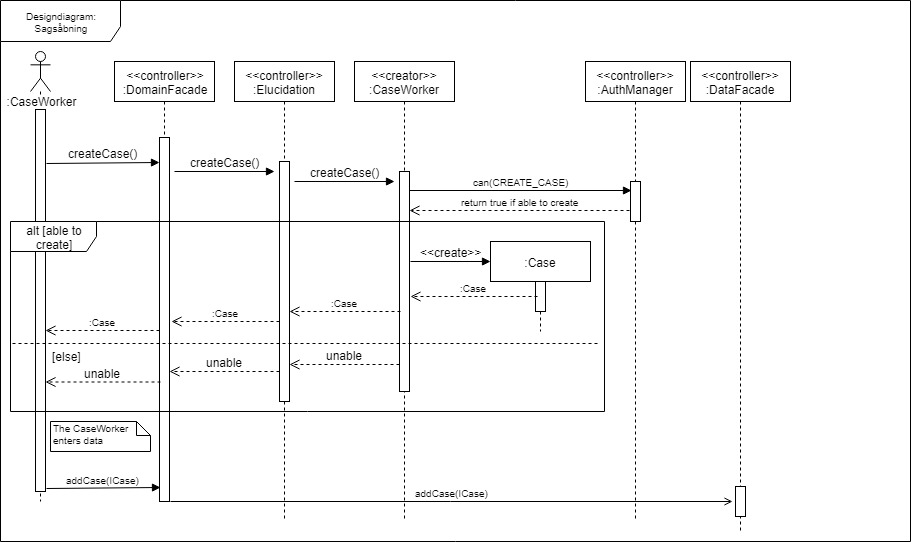
\includegraphics[scale=.45]{figurer/Sags_aabning_design.jpg}
  \caption{Designdiagram over hændelsesforløb for sagsåbbning brugsmønsteret}
  \label{fig:sags_aabning_design}
\end{figure}

På figur \ref{fig:sags_aabning_design} ses det, at \code{CaseWorker} starter hændelsesforløbet ved at oprette en sag med metoden \code{createCase()}. Dette diagram viser hvordan en sag oprettes, og tilføjes til den relationelle database. Ved at oprette dette diagram, kan der hurtigt skabes et overblik over livscyklusser for eksempel \code{createCase()}. På den måde kan der hurtigt fejlfindes i Sensum Udred eller ændres i metoder, fordi det vides i hvilke returtyper der skal ændres, eller hvilke metoder. Figur \ref{fig:login_design} viser design sekvensdiagrammet for login. Dette blev lavet for at have hændelsesforløb med implementeringsdetaljer.

\begin{figure}[H]
  \centering
  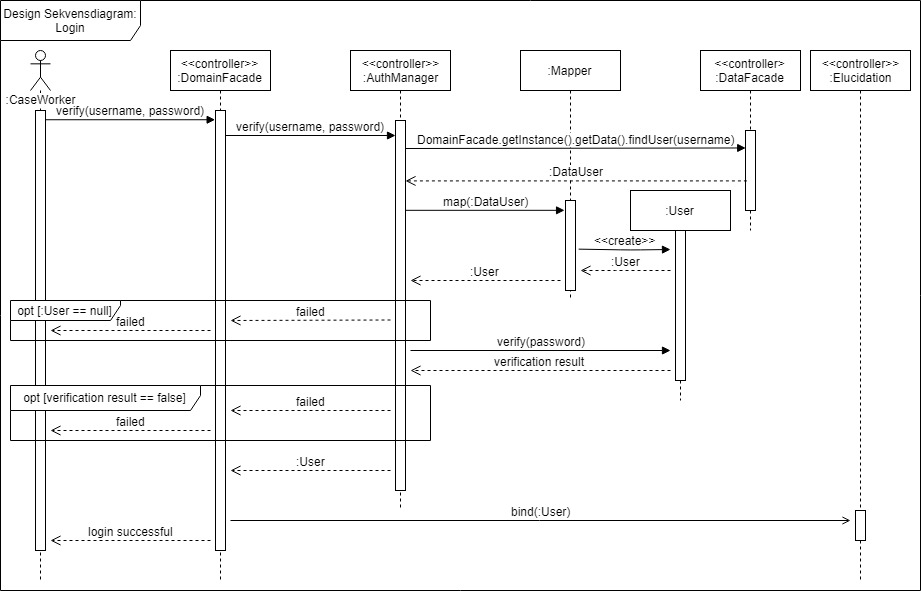
\includegraphics[scale=.45]{figurer/Login-Design-Sekvensdiagram.jpg}
  \caption{Designdiagram over hændelsesforløb for login brugsmønsteret}
  \label{fig:login_design}
\end{figure}

\paragraph{Arkitektonisk sekvensdiagram}\mbox{} \\
For at give et indblik i hvordan hændelsesforløbet foregår igennem lagene, er der lavet et arkitektonisk sekvensdiagram. Dette diagram har både GUI-laget, domain-laget og datalaget vist som pakker i diagrammet. På figur \ref{fig:arkitektonisk} kan diagrammet ses.

\begin{figure}[H]
  \centering
  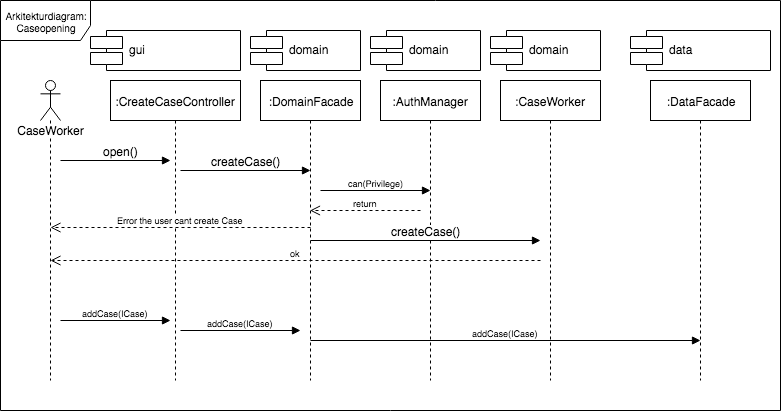
\includegraphics[scale=.42]{figurer/Sagsaabning.png}
  \caption{Arkitektonisk sekvensdiagram for sagsåbning}
  \label{fig:arkitektonisk}
\end{figure}

Diagrammet på figur \ref{fig:arkitektonisk} er med til at give et overblik over hele hændelsesforløbet for en \code{CaseWorker} helt oppe fra GUI-laget. Dette diagram hjalp med at se, om de rigtige metoder var implementeret i de rigtige lag. Et eksempel er, at der i diagrammet vises hvordan domainlaget står for, at oprette sagen, hvis \code{CaseWorker} har de rigtige privilegier. Dette blev ændret undervejs, da sagen i starten ikke fik tjekket privilegierk, og derfor kunne alle brugere af Sensum Udred oprette sager. Ved hjælp af dette diagram blev dette ændret, og \code{AuthManager} kom ind over, så det krævede privilegier for at kunne oprette en sag.

Det dynamiske view af designmodellen var med til at forbedre funktionaliteten af koden, da der iterativt blev arbejdet med diagrammer, og der derefter kunne tilføjes nye implementeringsdetaljer til designklassediagrammet. Det dynamiske view var derfor med til at finde fejl og mangler i Sensum Udred, men også forbedre Sensum Udred kodemæssigt. Helt basalt var fremgangsmåden for  denne del at arbejde iterativt, så der blev lavet et forsimplet designklassediagram, derefter sekvensdiagrammer, så tilbage og tilføje implementeringsdetaljer for at opnå den fulde funktionalitet.

\subsubsection{Arkitektur} \label{arkitektur}
Som et led i design processen er der overvejet hvordan projektets kode skal struktureres, for at opnå en god arkitektur i forhold til sikkerhed, vedligeholdelse og udvikling af Sensum Udred.

Måden hvorpå dette opnåes er ved at benytte en lagdelt arkitektur. Systemet skal opdeles i 3 overordnede lag \code{GUI}, \code{Domain} og \code{Data}. Hvert lag har hvert deres fokusområde. På denne måde kan vigtig funktionalitet indkapsles, og derved vil vedligeholdelse af systemet blive nemmere at håndtere, da ændringer i ét lag ikke vil påvirke de andre lags implementering. En lagdelt arkitektur giver også mulighed for, at et lag kan udskiftes undervejs For eksempel blev dette projektforløb startet med at implementere et simpelt \code{Data} lag, som senere blev erstattet med et der var mere avanceret. Kommunikations flowet i systemet går fra GUI til Domain til Data. Hvert lag har en facade klasse der eksponerer et api, som det øvre lag kan benytte til at påvirke laget under det. I nogle tilfælde vil det være nødvendigt at vende kommunikationsflowet da \code{GUI} kan spørge ned igennem lagene efter data. \code{Data} laget vil så returnere det fundne data op igennem igen til \code{GUI}. For at sikre, at der ikke er kobling på tværs af lagene, er der valgt at implementere Acquaintance. Dette er valgt, da det sikrer at der opnås en lav kobling på tværs af lagene, uden at gå på kompromis med at kunne eksponere entiteter på tværs af lagene. Facade klasserne i de forskellige lag skal alle implementeres som singletons. Dette sikrer at man ikke kan have flere instanser af hvert lag under runtime. På figur \ref{fig:arkitektur} ses et diagram over lagdeling  og kommunikationsflowet. \\

\begin{figure}[H]
  \centering
  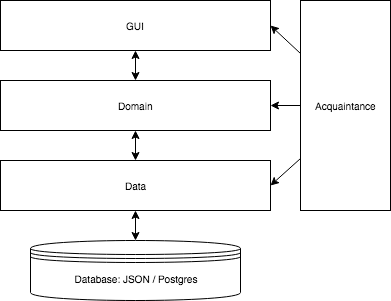
\includegraphics[scale=.6]{figurer/arkitektur.png}
  \caption{System arkitektur diagram}
  \label{fig:arkitektur}
\end{figure}


\subsubsection{Design af persistens}
For at fokusere på \code{Domain} lagets implementering i starten af elaborationsfasen, er det blevet valgt at \code{Data} laget i første iteration skulle implementeres som en simpel JSON database, der kunne gemme og læse en JSON-fil på den lokale harddisk.
	Hver entitet der skal gemmes i systemet har en klasse i pakken \code{data.model}. Entitets klasserne indeholder deres egen indkapslede data, samt implementering i forhold til hvordan den enkelte entitet kan gemme og hente dens data fra databasen. På figur \ref{fig:example_data_class} ses et eksempel på en data klasse der beskriver entiteten adresse i systemet. 
    Data klasser har en statisk \code{find(int id)} metode som udfra et id returnerer instanser med data hentet fra databasen. Data klasser kan oprettes eller opdateres med \code{save()} metoden, hvis instansen ikke allerede eksisterer i databasen vil den blive oprettet, ellers vil den udfra sit \code{id} blive opdateret. \\

\begin{figure}[H]
  \centering
  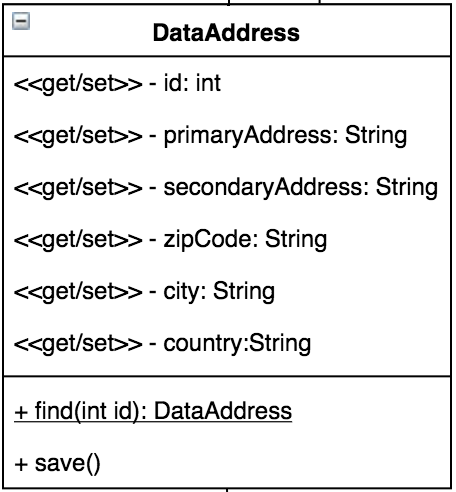
\includegraphics[scale=.6]{figurer/example_data_class.png}
  \caption{Eksempel af en data klasse der beskriver en adresse som en entitet i systemet}
  \label{fig:example_data_class}
\end{figure}

	I anden iteration i elaborationsfasen, blev JSON databasen udskiftet med en PostgreSQL database. Grunden til udskiftningen var, at PostgreSQL er bedre til at håndtere relationel data, og det giver også mulighed for at benytte SQL til filtrering og bearbejdning af data mere effektivt. 
    
\subsubsection{Database Design} \label{database-design}
I dette afsnit vil designvalg og overvejelser i forhold til strukturering af data i databasen blive forklaret.

   Databasens datastruktur er designet med fokus på, hvordan data optimalt og sikkert lagres i systemet. Her er der udfra principperne i \code{3rd normal form} kontrueret et database skema, så det undgås at have redundant data. Dette sikrer, at det gemte data ikke kommer ud af sync på tværs af tabeller, samt begrænser den data som bliver lagret, da det kun bliver gemt et enkelt sted, i modsætning til hvis det blev gemt i flere tabeller.
   Alle relationer i databasen er beskrevet i form af kolonnen \code{id}, som er et heltal andre tabeller kan referere til.
  
	For at få et bedre overblik over databasestrukturen, er der udarbejdet et relationelt database diagram, som kan ses på figur \ref{fig:er_diagram}. På diagrammet er de forskellige tabellers relationer beskrevet, samt hvilke kolonner de indeholder, og hvad deres data typer er. Ud fra det relationelle diagram kan det ses, at tabellen der indeholder information omkring personer eller firmaer har et en til en forhold til adresser. For eksempel har en person en adresse, og en adresse hører enten til en bestemt person eller firma. Et andet eksemple er, at en Borger kan have mange sager, men en sag kan kun høre til en enkelt borger. Derfor er dette forhold et mange til en. \\

\begin{figure}[H]
  \centering
  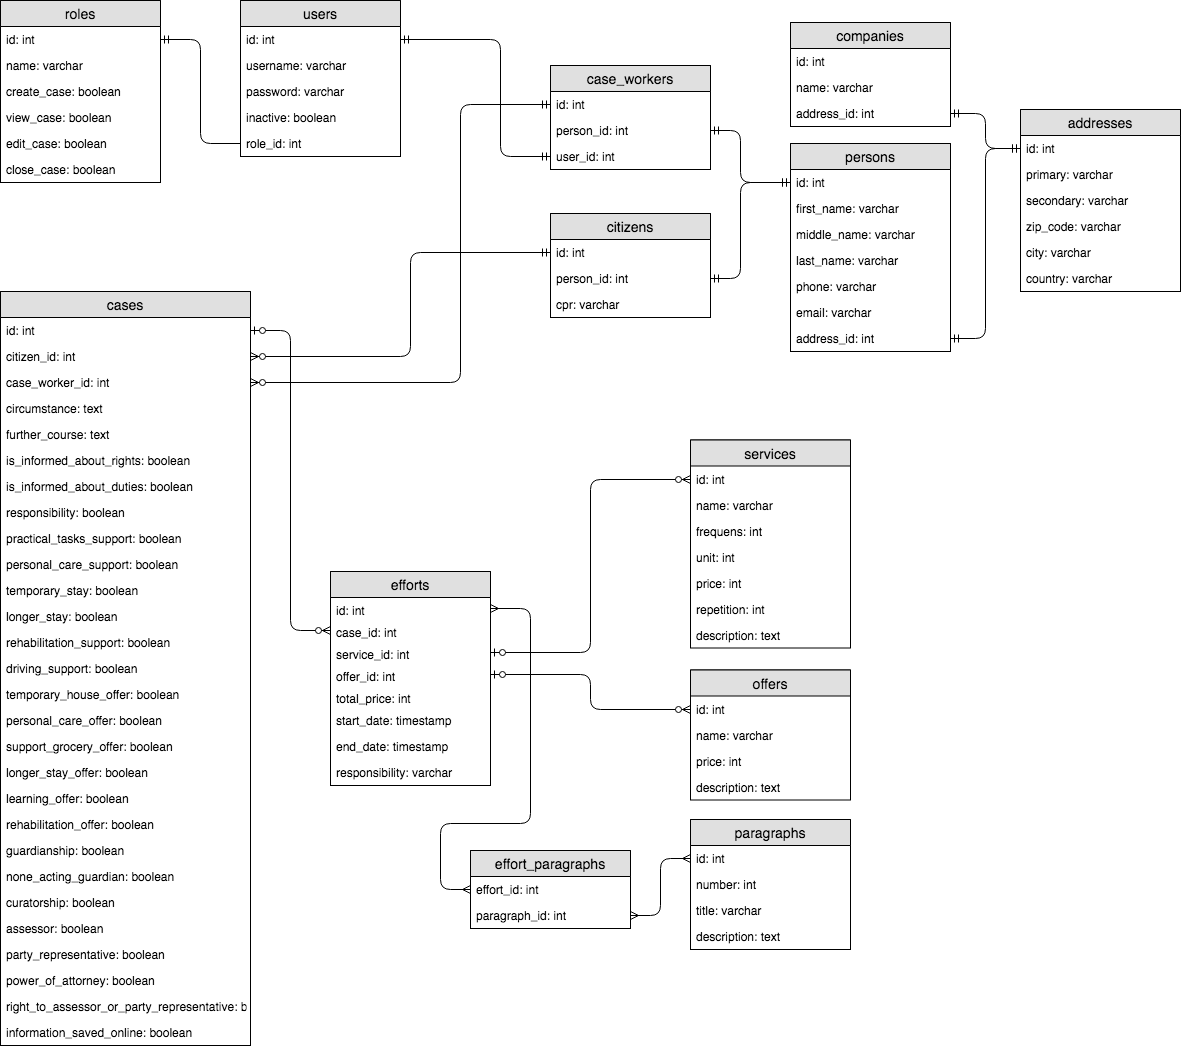
\includegraphics[scale=.30]{figurer/ER_Diagram.png}
  \caption{Relationelt diagram over database struktur}
  \label{fig:er_diagram}
\end{figure}

\end{document}